\documentclass[crop, tikz]{standalone}
\usepackage{tikz}

\usepackage{xcolor}
\definecolor{morange}{RGB}{255,127,14}
\definecolor{mblue}{RGB}{31,119,180}
\definecolor{mred}{RGB}{214,39,40}
\definecolor{mpurple}{RGB}{148,103,189}
\definecolor{mgreen}{RGB}{44,160,44}


\begin{document}

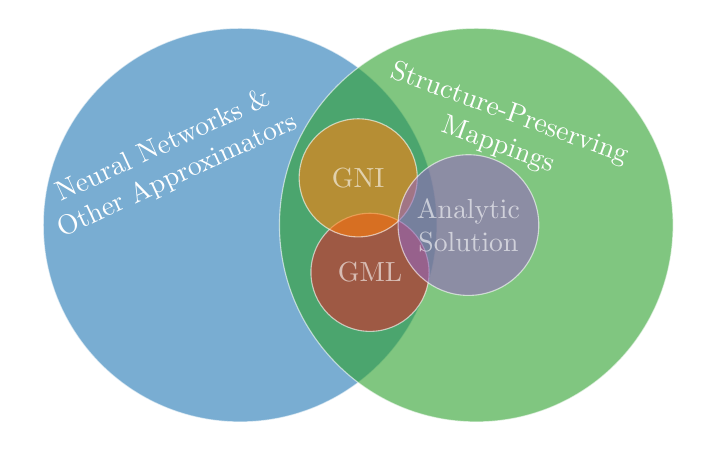
\begin{tikzpicture}[color=white]
  \tikzset{venn circle/.style={draw,circle,minimum width=5cm,fill=#1,opacity=0.6}}

  \node [venn circle = mblue, align=center] (A) at (0,0) {}; % A
  \node [anchor=north west, align = center, yshift = .5cm, xshift=-.2cm, rotate =25] at (A.west) {Neural Networks \& \\ Other Approximators};
  \node [venn circle = mgreen, align=center] (B) at (0:3cm) {}; % C
  \node [anchor=north west, align = center, yshift = -.25cm, xshift=-1.1cm, rotate=-20] at (B.north) {Structure-Preserving \\ Mappings};
  \node[venn circle = mred, minimum width=1.5cm, yshift=-.6cm, xshift=.15cm] at (barycentric cs:A=1/2,B=1/2 ) {GML}; 
  \node[venn circle = morange, minimum width=1.5cm, yshift=.6cm] at (barycentric cs:A=1/2,B=1/2 ) {GNI};
  \node[venn circle = mpurple, minimum width=1.5cm, xshift=1.4cm, align=center] at (barycentric cs:A=1/2,B=1/2 ) {Analytic \\ Solution};
\end{tikzpicture}  
\end{document}